

\chapter{Ways to Instruct Robots}
\label{chap:WaysToInstructRobots}
\minitoc
This chapter discusses the various ways in which the robot can be taught its task and how the interaction between humans and robots can be designed.
 
% \texttt{Intend task from scene}
\section{Scene Understanding}

The robot derives its task solely from the environment and the objects present in it and is not explicitly conditioned \cite{jang_BCZZeroShotTask_2022}. For example, if a teapot and a cup are present, the robot may infer that the task is to pour liquid from the teapot into the cup. This approach relies heavily on the robot's ability to understand the scene based on visual cues \cite{jang_BCZZeroShotTask_2022}.
% and infer the intended task based on visual cues and contextual information \cite{jang_BCZZeroShotTask_2022}. 
A distinction can be made between a policy that can identify and execute multiple tasks and a policy that can handle only a single task.

\paragraph{One Policy, Multiple Tasks}
In this setting, a single policy is typically specialized on a finite set of tasks. The policy must be explicitly trained for those tasks and tasks that are not represented or underrepresented in the training dataset, can therefore often not be executed reliably \cite{_BoostingRoboticManipulation_, mandi_CACTIFrameworkScalable_2023}. For example, if the policy has been trained on multiple manipulation tasks and one of them involves pouring liquid from a teapot into a cup, the policy will execute this behavior when a matching scene is observed during inference \cite{jang_BCZZeroShotTask_2022}.
However, generalization to other objects or situations is often limited. Using different teapots or cups may not be problematic as long as the relevant visual features are recognized. In contrast, performance typically decreases under significantly different objects or scenes \cite{jang_BCZZeroShotTask_2022}. 
% If a corresponding pouring behavior from a cooking pot was not included during training, the policy may fail to transfer the action to that new object category \cite{_BoostingRoboticManipulation_, jang_BCZZeroShotTask_2022}.
A major limitation of this approach is task ambiguity caused by overlapping object context across different behaviors. If the same object types, such as a teapot and a cup, appear in both a pick-and-place task and a pouring task, the policy may not be able to disambiguate the correct action target based on scene context alone \cite{tamar_IMITATIONLEARNINGVISUAL_2018}.


\paragraph{One Policy, One Task}
An alternative approach is to train a separate policy for each individual task, which is then selected explicitly during inference. 
The task-specific policy selection can be performed either manually by a human or automatically by a separate \ac{AI} classification model that analyzes the scene and determines the appropriate policy \cite{chen_RoboRouterTrainingFreePolicy_2026}. For example, one policy could be trained for ``pouring'', another for ``opening a drawer''. This modular design is closely related to task-aware expert routing and decoupled planning-and-execution frameworks in robotic manipulation \cite{chen_RoboRouterTrainingFreePolicy_2026}.
This decoupling enables training each policy on significantly larger and more diverse datasets containing varied object appearances and environmental conditions, while keeping the core task semantics fixed \cite{raffin_DECOUPLINGFEATUREEXTRACTION_2019}. Consequently, these specialized policies often support more robust generalization across novel object instances and environmental variations compared to the \textit{One Policy, Multiple Tasks} paradigm. \cite{bai_LearningSeeAct_2025, _MultitaskRobotManipulation_a, tamar_IMITATIONLEARNINGVISUAL_2018}





\section{Language Instructions}

For humans, the most comfortable way to instruct the robot is with voice commands. This is very useful for simple tasks that are easy to summarize. But complex tasks, where execution must follow exact instructions, are sometimes difficult to describe in words \cite{Jain2024Vid2RobotEV}. For example, how would you teach a humanoid robot to decorate tables exactly like a sample table, especially when various decorations need to be assembled in a complex arrangement?
Furthermore ambiguities may arise, and the same instruction may be interpreted differently according to the linguistic context. For example, the word ``open'' is used for: open drawer, open cabinet, open container with lid or open jar with screw cap. Although the same verb is used here, each interaction requires a completely different motor control \cite{Jain2024Vid2RobotEV}.
Commanding the robot with voice commands enables an interactive dialogue between humans and the robot. If the robot does not understand the instructions, it can ask follow-up questions to clarify any misunderstandings. This helps minimize the problems associated with voice commands.



\section{Image Instructions}

Robots can also be instructed using visual inputs such as images. Compared to language, image-based instructions provide a more concrete and unambiguous specification of spatial arrangements, object relations and desired outcomes.

A common approach is the use of \textbf{goal images}, where the robot is given a visual representation of the desired final state. The robot observes the current state and acts such that it minimizes the difference to the goal image. This is often referred to as goal-conditioned behavior. However, this approach does not explicitly specify \textit{how} the task should be executed, only \textit{what} the final configuration should look like. But some works have addressed this issue with the usage of annotations in the image of the initial state to specify the task execution. For example \cite{bai_LearningSeeAct_2025} highlights the relevant objects and regions with circles and arrows to visualize the task execution in the image, see \autoref{fig:ImageInstructions}. 
Another way to address this limitation, \textbf{subgoal images} or intermediate states can be provided \cite{pathak_ZeroShotVisualImitation_2018}. These guide the robot through a sequence of visually defined steps, effectively decomposing complex tasks into simpler stages. This is particularly useful for long-horizon or multi-step manipulation tasks.

\begin{figure}[h]
	\centering
	\subfigure[Task: Rotate cup and place it on table]{
		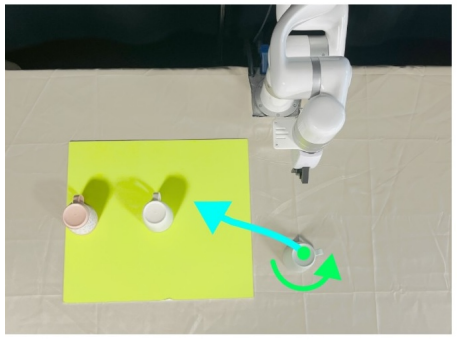
\includegraphics[width=4.5cm]{./chapter4/media/ImageInstruction_1}
		\label{fig:ImageInstruction_1}
	}
	\hspace{0.5cm}
	\subfigure[Task: Put fruit into bowl]{
		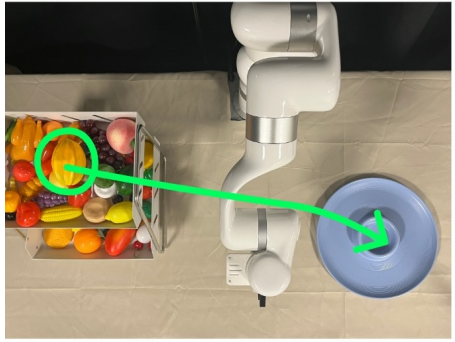
\includegraphics[width=4.5cm]{./chapter4/media/ImageInstruction_2}
		\label{fig:ImageInstruction_2}
	}
	\hspace{0.5cm}
	\subfigure[Task: Fold T-shirt]{
		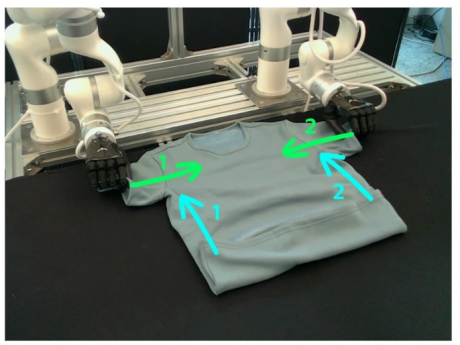
\includegraphics[width=4.5cm]{./chapter4/media/ImageInstruction_3}
		\label{fig:ImageInstruction_3}
	}
	\caption[Image-based instructions for task execution.]{Image-based instructions for task execution: Highlighting relevant objects and regions with circles and arrows to visualize the task execution. Image source: \cite{bai_LearningSeeAct_2025}.}
    \label{fig:ImageInstructions}
\end{figure}

A key advantage of image instructions is their ability to capture fine-grained spatial details that are difficult to describe in language, such as precise object placement, orientation or symmetry alignments. However, they also introduce challenges related to perception, such as viewpoint variation, occlusions of objects in the real environment, or the use of in-the-wild goal-images with varying lighting and background conditions.




\section{Video-Based Instructions}

Demonstration videos are a powerful way to instruct robots, as they contain rich visual and temporal information. In contrast to single images, videos provide not only the desired goal state of a task but also the sequence of intermediate steps required to reach that goal \cite{Jain2024Vid2RobotEV}.
In this setting, the task is typically formulated as an \ac{IL} problem, where the robot learns a policy that maps visual observations to actions by imitating the demonstrated trajectory \cite{Jain2024Vid2RobotEV}. The temporal structure of the video enables the robot to infer \textit{how} a task should be executed, rather than only \textit{what} the final outcome should look like. Depending on the setup, this may also require inferring latent actions from visual observations alone \cite{Jain2024Vid2RobotEV}.
Ideally, the robot model should be able to understand it's task from in-the-wild demonstration videos of both robots and humans \cite{Chen2025VidBotLG}. Such data exhibits large variability in lighting, backgrounds, and camera motion, making it significantly more challenging for perception and learning compared to controlled laboratory data.
% In-the-wild videos refer to video data collected in unconstrained, real-world environments, without controlled settings, standardized viewpoints, or curated conditions.

Demonstration videos from humans and robots differ in their characteristics and are challenging for learning. In addition, a third category ``teleoperation'' is being introduced, which is often used for fine-tuning the robot. There a human directly controls the robot to generate demonstrations.
The following sections discuss the specific advantages and challenges of each type of demonstration video.

\paragraph{Human Video Demonstrations}
Human demonstrations videos are a natural and intuitive way to teach robots.  However, these videos are commonly Raw RGB or RGB-D videos with depth, which lack explicit on action labels and trajectory data. 
The characteristics of human demonstration videos are:
\begin{itemize}
	% In this paradigm, the robot learns from videos of humans performing a task. This is particularly appealing, as l
	\item \textbf{Data Abundance:} Large amounts of human demonstration data are readily available on the internet \cite{McCarthy_2025, Eze2024LearningBW}. 
	\item \textbf{Embodiment Gap:} A core challenge is the mismatch between human and robot bodies. Human motions and kinematics differ significantly from those of robots and the robot must learn to map observed human actions to its own action space \cite{McCarthy_2025}.
	\item \textbf{Suboptimal Demonstrations:} Another key challenge of human video demonstrations is that they do not necessarily represent optimal task executions. Demonstrations often reflect individual preferences, inefficiencies, or context-specific behaviors, resulting in suboptimal trajectories. In many cases, a video captures only a single possible way of solving the task without providing information about alternative or more efficient strategies. However, the objective for the robot is typically to perform tasks efficiently and robustly. Therefore, the learned policy must be able to generalize beyond the demonstrated behavior and, if necessary, improve upon it, rather than directly imitating potentially suboptimal actions \cite{McCarthy_2025}.
\end{itemize}






\paragraph{Robot Video Demonstrations With No Trajectory Information}
RGB and RGB-D robot demonstration videos lack, like human videos on action labels and trajectory data too, but with the difference that the robot is performing the demonstration. These videos are recorded from the robot's perspective or a stationary camera. This also includes demonstrations in which a person operates with a robotic arm in their hand or holds a robotic gripper to perform tasks. The characteristics of robot demonstrations videos are:
\begin{itemize}
	\item \textbf{No Embodiment Gap:} The demonstrations are performed by the robot itself or by another robot with similar embodiment. This avoids the human-robot embodiment gap and provides more directly transferable data \cite{McCarthy_2025}. 
	\item \textbf{Cost and Effort:} Collecting robot demonstrations is often expensive and time-consuming, as it requires access to robotic systems and typically controlled environments. In addition, purely visual robot demonstrations may still lack explicit action labels. This means that the robot must still infer the underlying actions and intentions from the visual data \cite{McCarthy_2025}. 
	\item \textbf{Value of Robot Demos:} Despite these challenges, robot video demonstrations can provide valuable data for learning, as they are more closely aligned with the robot's own capabilities and constraints compared to human demonstrations \cite{McCarthy_2025}.
\end{itemize}



\paragraph{Teleoperation}
Teleoperation videos contain not only visual observations but also trajectory and action information. 
The demonstrations are generated by directly controlling the robot, e.g. via a joystick or a dedicated control interface \cite{McCarthy_2025}.
%  and all trajectory information are recorded \cite{McCarthy_2025}.
\begin{itemize}
	% \item \textbf{Direct Data Collection:} A common method to generate high-quality robot demonstrations is teleoperation, where a human operator directly controls the robot, e.g. via a joystick or a dedicated control interface \cite{McCarthy_2025}.
	\item \textbf{Precision and Safety:} 
	% In contrast to passive video demonstrations, teleoperation provides access to both the visual observations and the corresponding action and trajectory data. As a result, 
	The demonstrated actions are already expressed in the robot's action space, which significantly simplifies reproducing the expected behavior. Such demonstrations are particularly important for fine-grained manipulation tasks that require precise control and accurate timing  \cite{McCarthy_2025}. 
	\item \textbf{Scalability Issues:} However, teleoperation may require specialized hardware (controllers, sometimes motion-capture or VR setups) and does not scale as easily as collecting passive video data. Thus, collecting large teleoperation datasets can be time-consuming and is typically done in lab settings only \cite{McCarthy_2025}.
\end{itemize}

